  \solution{
Implication graph:\medskip

%TCIMACRO{%
%\TeXButton{Decision tree}{\begin{tikzpicture}[node distance=2.5cm,auto]
%\node (A) {A=0@1};
%\node (B) [right of=A] {B=1@1};
%\node (D) [right of=B] {D=0@3};
%\node (G) [right of=D] {G=0@3};
%\node (H) [below of=G] {H=1@3};
%\node (K) [right of=H] {$\mathcal K$};
%\node (E) [above of=D] {E=0@3};
%\node (F) [right of=E] {F=1@3};
%\node (J) [right of=G] {J=1@3};
%\node (C) [above of=J] {C=1@2};
%\path[->] (A) edge node {$c_1$} (B);
%\path[->] (B) edge node {$c_3$} (D);
%\path[->] (D) edge node {$c_5$} (G);
%\path[->] (G) edge node {$c_2$} (H);
%\path[->] (H) edge node {$c_7$} (K);
%\path[->] (A) edge node {$c_2$} (H);
%\path[->] (C) edge node {$c_6$} (J);
%\path[->] (J) edge node {$c_7$} (K);
%\path[->] (E) edge node {$c_3$} (D);
%\path[->] (E) edge node {$c_4$} (F);
%\path[->] (F) edge node {$c_5$} (G);
%\path[->] (G) edge node {$c_6$} (J);
%\end{tikzpicture}}}%
%BeginExpansion
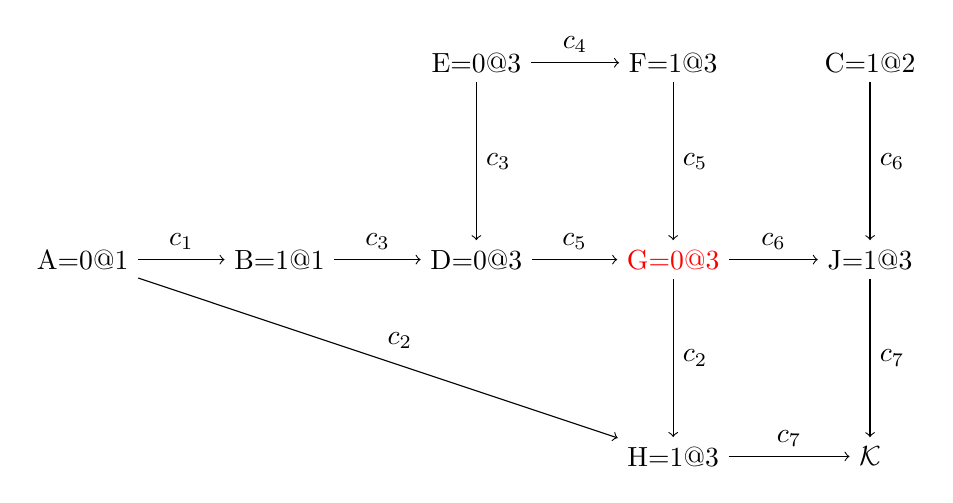
\begin{tikzpicture}[node distance=2.5cm,auto]
\node (A) {A=0@1};
\node (B) [right of=A] {B=1@1};
\node (D) [right of=B] {D=0@3};
\color{red}
\node (G) [right of=D] {G=0@3};
\color{black}
\node (H) [below of=G] {H=1@3};
\node (K) [right of=H] {$\mathcal K$};
\node (E) [above of=D] {E=0@3};
\node (F) [right of=E] {F=1@3};
\node (J) [right of=G] {J=1@3};
\node (C) [above of=J] {C=1@2};
\path[->] (G) edge node {$c_6$} (J);
\path[->] (F) edge node {$c_5$} (G);
\path[->] (C) edge node {$c_6$} (J);
\path[->] (J) edge node {$c_7$} (K);
\path[->] (E) edge node {$c_3$} (D);
\path[->] (E) edge node {$c_4$} (F);

\path[->] (A) edge node {$c_1$} (B);
\path[->] (B) edge node {$c_3$} (D);
\path[->] (D) edge node {$c_5$} (G);
\path[->] (G) edge node {$c_2$} (H);
\path[->] (H) edge node {$c_7$} (K);
\path[->] (A) edge node {$c_2$} (H);
\end{tikzpicture}%
%EndExpansion
\newline
Implication Graph with first UIP (red) and the corresponding cuts (dashed).\\
\bigskip

We have a conflict in $c_7$, since $\neg J$ and $\neg H$ are not satisfied.
So we have to resolve and backtrack to the first UIP (which is $G=0@3$).\\
Since $c_2$, $c_6$ and $c_7$ are conflict clauses along the out-edges and are
the first on the paths from the first UIP. Then the assertion clause can be
computed, using resolution as follows:\\
\\
$c_2: A \OR G \OR H$\\
\underline{$c_7: \neg J \OR \neg H$}\\
$c_8: A \OR G \OR \neg J$\\

$c_6: \neg C \OR G \OR J$\\
\underline{$c_8: A \OR G \OR \neg J$}\\
$c_9: A \OR \neg C \OR G$ (after removing the second G with fac.)\\
\\
Thus, this yields the resulting learned clause $c_9 = (A \OR \neg C \OR G)$
and we backtrack to the highest decision level ($DL = 3$), i. e. we delete decisions
and values at $DL 3$ and change the decision of $E$ to $E = 1@3$.\\
\\
So we get the new implication graph:\\

%TCIMACRO{%
%\TeXButton{Decision tree}{\begin{tikzpicture}[node distance=2.5cm,auto]
%\node (A) {A=0@1};
%\node (B) [right of=A] {B=1@1};
%\node (C) [right of=B] {C=1@2};
%\node (E) [right of=C] {E=1@3};	
%\path[->] (A) edge node {$c_1$} (B);
%\end{tikzpicture}}}%
%BeginExpansion
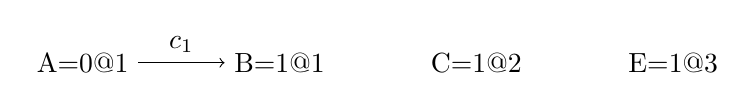
\begin{tikzpicture}[node distance=2.5cm,auto]
\node (A) {A=0@1};
\node (B) [right of=A] {B=1@1};
\node (C) [right of=B] {C=1@2};
\node (E) [right of=C] {E=1@3};				
\path[->] (A) edge node {$c_1$} (B);
\end{tikzpicture}%
%EndExpansion
\newline
\\
The remaining clauses $c_2$, $c_5$, $c_6$ and $c_7$ doesn't contain any rules
for the implication graph, so we have to introduce a new decision level $DL 4$
and we can choose the decision for e. g. $G$ as $G = 1@4$:\\
\bigskip

%TCIMACRO{%
%\TeXButton{Decision tree}{\begin{tikzpicture}[node distance=2.5cm,auto]
%\node (A) {A=0@1};
%\node (B) [right of=A] {B=1@1};
%\node (C) [right of=B] {C=1@2};
%\node (E) [right of=C] {E=1@3};
%\node (G) [right of=E] {G=1@4};	
%\path[->] (A) edge node {$c_1$} (B);
%\end{tikzpicture}}}%
%BeginExpansion
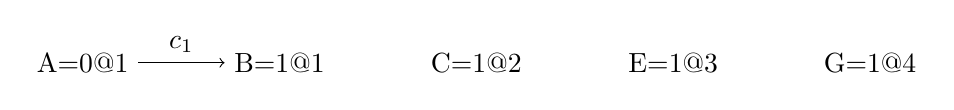
\begin{tikzpicture}[node distance=2.5cm,auto]
\node (A) {A=0@1};
\node (B) [right of=A] {B=1@1};
\node (C) [right of=B] {C=1@2};
\node (E) [right of=C] {E=1@3};	
\node (G) [right of=E] {G=1@4};			
\path[->] (A) edge node {$c_1$} (B);
\end{tikzpicture}%
%EndExpansion
\newline
\\
Again, the remaining clauses $c_5$ and $c_7$ doesn't contain any rules
for the implication graph, so we have to introduce a new decision level two
times ($DL 5$ and $DL 6$) and we can choose the decisions for e. g. $D$ as 
$D = 1@5$ and $H$ as $H = 0@6$:\\
\bigskip

%TCIMACRO{%
%\TeXButton{Decision tree}{\begin{tikzpicture}[node distance=2.5cm,auto]
%\node (A) {A=0@1};
%\node (B) [right of=A] {B=1@1};
%\node (C) [right of=B] {C=1@2};
%\node (E) [right of=C] {E=1@3};
%\node (G) [right of=E] {G=1@4};	
%\node (D) [below right of=A] {D=1@5};
%\node (H) [below right of=C] {H=0@6};
%\path[->] (A) edge node {$c_1$} (B);
%\end{tikzpicture}}}%
%BeginExpansion
\begin{tikzpicture}[node distance=2.5cm,auto]
\node (A) {A=0@1};
\node (B) [right of=A] {B=1@1};
\node (C) [right of=B] {C=1@2};
\node (E) [right of=C] {E=1@3};	
\node (G) [right of=E] {G=1@4};	
\node (D) [below right of=A] {D=1@5};
\node (H) [below right of=C] {H=0@6};		
\path[->] (A) edge node {$c_1$} (B);
\end{tikzpicture}%
%EndExpansion
\newline
Now we have fulfilled all clauses $c_i$, $i \in \{1,...,9\}$ and therefore we can
choose any dedcisions for the ramaining values.\\
A valid solution would be: $\{\neg A, B, C, D, E, F, G, \neg H, J\}$
\bigskip

%\node (K) [right of=H] {$\mathcal K$};
%\node (F) [right of=E] {F=1@3};
%\node (J) [right of=G] {J=1@3};		

  }